\begin{figure}[t!]
    \centering
    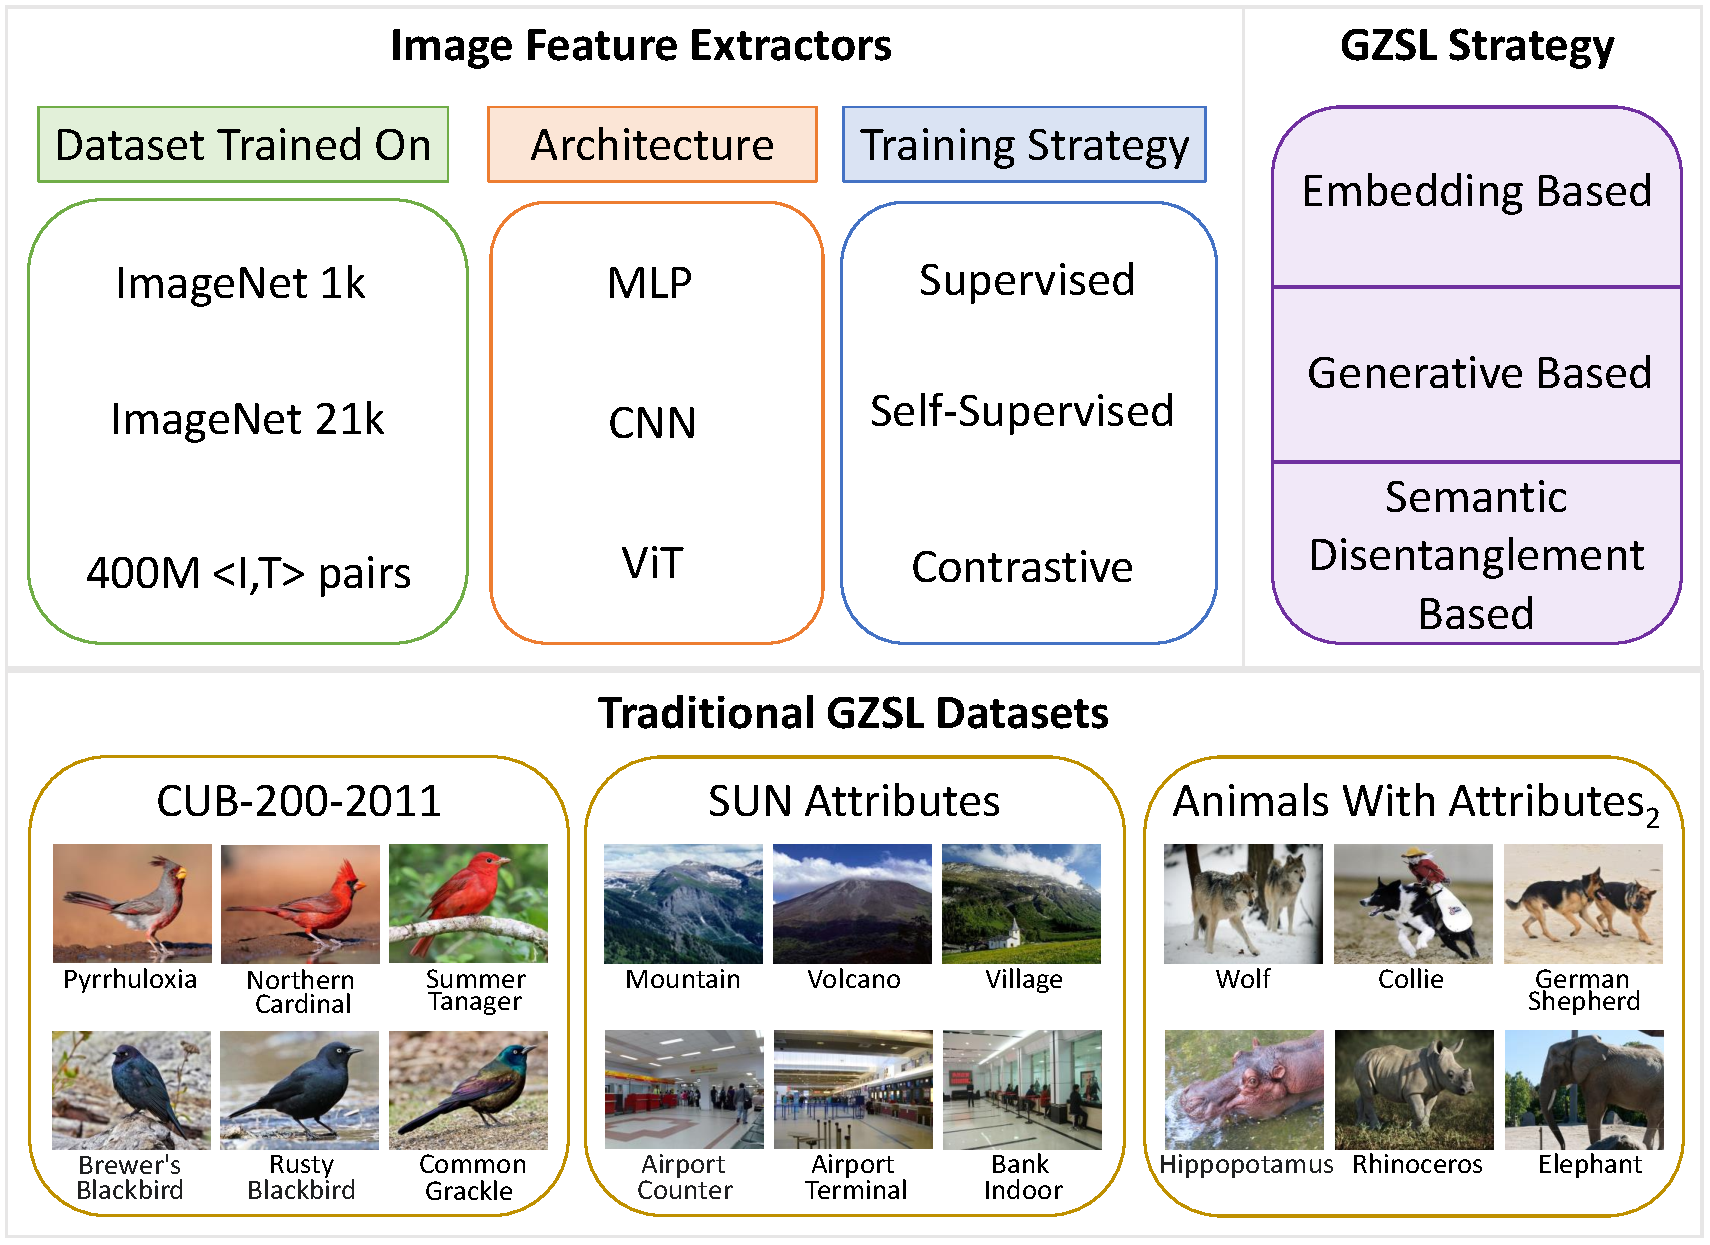
\includegraphics[width=\linewidth]{Images/FIG1_CVPR.pdf}
    \caption{\textbf{Overview of our large-scale analysis.} We explore a diverse set of visual feature backbones that were trained using different objectives. We further use them to extract visual features and train a diverse set of classic and modern Generalized Zero-shot Learning (GZSL) methods. We use three standard datasets to measure the methods' performance: CUB-200-2011 and SUN Attributes, which are fine-grained, and Animales with Attributes 2 (AWA2) which is a coarse-grained dataset. Best viewed in color.}
    \label{fig:figure1}
    \vspace{-0.1in}
\end{figure}

\section{Introduction}

Deep learning models have achieved remarkable accuracy in many computer vision classification tasks when labeled data is available, and the data distribution is consistent during training and test time~\cite{effectivenessData, revisitEffectivenessData, Ren2015FasterRT}. It is now possible to train image classifiers that can distinguish with high accuracy thousands of image categories~\cite{Russakovsky2015ImageNetLS}. 
However, in order to enable a model to recognize novel categories, it is still necessary to collect a dataset with representative human-labeled examples.
For this reason, literature has proposed zero-shot learning to help a model recognize novel {\em unseen} categories without needing any images of the new category. Zero-shot learning relies on auxiliary information such as textual descriptions or category attributes~\cite{5206772,elhoseiny2013write,lampert2013attribute}. 
The general idea is to leverage the auxiliary information to transfer visual knowledge from images in {\em seen} categories to a set of images from {\em unseen} categories. 
Once this function is learned, it can be used to categorize {\em unseen} samples into novel classes.


Early work on zero-shot learning focused on obtaining a good accuracy just on a set of {\em unseen} categories at inference time. In a more challenging scenario known as Generalized Zero-shot Learning (GZSL), both {\em seen} and {\em unseen} categories are considered at test time~\cite{Chao2016AnES, Pourpanah2020ARO}. This setup is more realistic and has been adopted in all the recent works in zero-shot learning; therefore, we focus exclusively on this setting.

First-generation methods are coined as embedding-based techniques, which focus on learning a function to align the seen images and unseen attributes and further measure the similarity between the mapped and predicted representations of the data samples in the embedding space~\cite{ESZSL, ALE, Zhang2017LearningAD, Zhang2020TowardsED}.
Further GZSL methods have shown significant improvement over this early work by teaching a model to generate the visual features of the {\em unseen} classes based on the visual features of the {\em seen} classes and the semantic representations of both {\em seen} and {\em unseen} categories. 
More recent works have instead explored rich image feature representations and their ability to provide enough information for a mapping function to generalize to new classes~\cite{Tong2019HierarchicalDO, SDGZSL}. 
These methods propose to learn discriminative representations from image features through disentanglement over feature groups by factorizing the useful dimensions to avoid bias towards the seen categories when trying to learn an attribute-visual alignment.

While disentanglement-based methods have significantly improved over prior work,
the representation capabilities of image features have mostly been tested under a ResNet101 model~\cite{RNs} pre-trained on Imagenet~\cite{AWA2, Liu2018GeneralizedZL}. 
In this work, we propose to explore different architectures trained with different objectives to be used as feature extractors. Given the wide availability of pre-trained model parameters~\cite{Gavrikov2022CNNFD, timm, Croce2021RobustBenchAS}, we perform a large-scale analysis to assess the impact of modern visual features backbones, our results are summarized in Figure~\ref{fig:figure1}. 
In our analysis, we consider visual features extracted from both uni-modal and multi-modal architectures pre-trained on standard settings, i.e., models pre-trained with ImageNet-1K; to models pretrained with even larger amounts of data, i.e., models pre-trained with ImageNet-21K and models pre-trained with 400 million Image/Text pairs.

Our results show that ResNet101 and similar feature extractors may not provide enough information, given the nature of the backbone architecture limitations and the training objective. 
Moreover, when examining feature extractors pre-trained with larger datasets, one would assume that the features extracted would contain more similarities to the data present in the GSZL test splits, causing all methods to perform better due to data leakage. However, we found that using features extracted from large-scale pre-trained {\em uni-modal networks} does not significantly impact the zero-shot performance.
Our experiments also reveal that with feature representations extracted from Visual Transformer~\cite{ViT} based architectures, no semantic disentanglement module is necessary to achieve state-of-the-art performance, and generative-based methods are superior in all benchmarks by a large margin ($\approx23\%$) when using features extracted from Transformer based architectures~\cite{ViT} trained with a contrastive objective.
Furthermore, given the capabilities of new models~\cite{CLIP, ALIGN, Singh2022FLAVAAF} to generalize to new tasks, we investigate how CLIP~\cite{CLIP} performs against GZSL methods and reveal that generative-based GZSL techniques are still necessary to achieve state-of-the-art results on fine-grained datasets.


Our primary contributions can be summarized as follows:


\begin{compactitem}
\item A large-scale study of different methods and features extracted from a diverse set of architectures and training approaches, applied to state-of-the-art methods from different GZSL families (i.e., embedding based~\cite{ALE, ESZSL, DeViSE}, generative based~\cite{tfvaegan, CADA_VAE, CE}, semantic disentanglement based~\cite{Tong2019HierarchicalDO, Chen2021FREE, SDGZSL}). 


\item A library containing the revisited GSZL methods we chose to explore, allowing a unified codebase for reproducibility and further analysis based on the findings shown in this work. Texts generated to finetune the models based on the attribute vectors provided in each dataset, along with the weights and the extracted features we use in our experiments.

\item Updates and key insights which we hope will reshape the Generalized Zero-Shot Learning research track in favor of leveraging richer feature representations. 

\end{compactitem}

We expect our work to motivate further feature representation explorations to the GZSL task in a more realistic, practical, and challenging scenario, given the recent advances with large pre-trained models. All the resources used, including GPU information and computing infrastructure are detailed in the Appendix, along with hyperparameter selections and data splits we use for all our experiments.

%%%%%%%%%%%%%%%%%%%%%%